%%%%%%%%%%%%%%%%%%%%%%%%%%%%%%%%%%%%%%%%%
% Wenneker Assignment
% LaTeX Template
% Version 2.0 (12/1/2019)
%
% This template originates from:
% http://www.LaTeXTemplates.com
%
% Authors:
% Vel (vel@LaTeXTemplates.com)
% Frits Wenneker
%
% License:
% CC BY-NC-SA 3.0 (http://creativecommons.org/licenses/by-nc-sa/3.0/)
% 
%%%%%%%%%%%%%%%%%%%%%%%%%%%%%%%%%%%%%%%%%

%----------------------------------------------------------------------------------------
%	PACKAGES AND OTHER DOCUMENT CONFIGURATIONS
%----------------------------------------------------------------------------------------

\documentclass[11pt]{scrartcl} % Font size

%%%%%%%%%%%%%%%%%%%%%%%%%%%%%%%%%%%%%%%%%
% Wenneker Assignment
% Structure Specification File
% Version 2.0 (12/1/2019)
%
% This template originates from:
% http://www.LaTeXTemplates.com
%
% Authors:
% Vel (vel@LaTeXTemplates.com)
% Frits Wenneker
%
% License:
% CC BY-NC-SA 3.0 (http://creativecommons.org/licenses/by-nc-sa/3.0/)
% 
%%%%%%%%%%%%%%%%%%%%%%%%%%%%%%%%%%%%%%%%%

%----------------------------------------------------------------------------------------
%	PACKAGES AND OTHER DOCUMENT CONFIGURATIONS
%----------------------------------------------------------------------------------------

\usepackage{amsmath, amsfonts, amsthm} % Math packages

\usepackage{listings} % Code listings, with syntax highlighting

\usepackage[czech]{babel}

\usepackage{graphicx} % Required for inserting images
\graphicspath{{Figures/}{./}} % Specifies where to look for included images (trailing slash required)

\usepackage{booktabs} % Required for better horizontal rules in tables

\numberwithin{equation}{section} % Number equations within sections (i.e. 1.1, 1.2, 2.1, 2.2 instead of 1, 2, 3, 4)
\numberwithin{figure}{section} % Number figures within sections (i.e. 1.1, 1.2, 2.1, 2.2 instead of 1, 2, 3, 4)
\numberwithin{table}{section} % Number tables within sections (i.e. 1.1, 1.2, 2.1, 2.2 instead of 1, 2, 3, 4)

\setlength\parindent{0pt} % Removes all indentation from paragraphs

\usepackage{enumitem} % Required for list customisation
\setlist{noitemsep} % No spacing between list items

% clickable links
\usepackage{hyperref}

%----------------------------------------------------------------------------------------
%	DOCUMENT MARGINS
%----------------------------------------------------------------------------------------

\usepackage{geometry} % Required for adjusting page dimensions and margins

\geometry{
	paper=a4paper, % Paper size, change to letterpaper for US letter size
	top=2.5cm, % Top margin
	bottom=3cm, % Bottom margin
	left=3cm, % Left margin
	right=3cm, % Right margin
	headheight=0.75cm, % Header height
	footskip=1.5cm, % Space from the bottom margin to the baseline of the footer
	headsep=0.75cm, % Space from the top margin to the baseline of the header
	%showframe, % Uncomment to show how the type block is set on the page
}

%----------------------------------------------------------------------------------------
%	FONTS
%----------------------------------------------------------------------------------------

\usepackage[utf8]{inputenc} % Required for inputting international characters
\usepackage[T1]{fontenc} % Use 8-bit encoding

\usepackage{fourier} % Use the Adobe Utopia font for the document

%----------------------------------------------------------------------------------------
%	SECTION TITLES
%----------------------------------------------------------------------------------------

\usepackage{sectsty} % Allows customising section commands

\sectionfont{\vspace{6pt}\centering\normalfont\scshape} % \section{} styling
\subsectionfont{\normalfont\bfseries} % \subsection{} styling
\subsubsectionfont{\normalfont\itshape} % \subsubsection{} styling
\paragraphfont{\normalfont\scshape} % \paragraph{} styling

%----------------------------------------------------------------------------------------
%	HEADERS AND FOOTERS
%----------------------------------------------------------------------------------------

\usepackage{scrlayer-scrpage} % Required for customising headers and footers

\ohead*{} % Right header
\ihead*{} % Left header
\chead*{} % Centre header

\ofoot*{} % Right footer
\ifoot*{} % Left footer
\cfoot*{\pagemark} % Centre footer
 % Include the file specifying the document structure and custom commands

%----------------------------------------------------------------------------------------
%	TITLE SECTION
%----------------------------------------------------------------------------------------

\title{	
	\normalfont\normalsize
	\textsc{ČVUT, Fakulta informačních technologií}\\ % Your university, school and/or department name(s)
	\textsc{Vyhledávání na webu a v multimediálních databázích}\\
	\textsc{Letní semestr 2019/2020}\\
	\textsc{Závěrečná zpráva k projektu}\\
	\vspace{25pt} % Whitespace
	\rule{\linewidth}{0.5pt}\\ % Thin top horizontal rule
	\vspace{20pt} % Whitespace
	{\huge LSI vektorový model}\\ % The assignment title
	\vspace{12pt} % Whitespace
	\rule{\linewidth}{2pt}\\ % Thick bottom horizontal rule
	\vspace{12pt} % Whitespace
}

\author{\LARGE David Mašek a Kristýna Klesnilová} % Your name
\date{\normalsize\today} % Today's date (\today) or a custom date

\begin{document}

\maketitle % Print the title

\newpage

\tableofcontents

\newpage

\section{Popis projektu}

V tomto projektu implementujeme \emph{LSI vektorový model} sloužící k podobnostnímu vyhledávání v databázi anglických textových dokumentů. Tuto funkcionalitu následně vizualizujeme pomocí webového interface, který uživateli umožňuje procházet databázi článků na základě doporučování nejpodobnějších článků k právě čtenému.

\bigskip 

V experimentální části projektu jsme se dále zaměřili na:
\begin{itemize}
	\item Určení optimálního počtu konceptů
	\item Porovnání vlivu LSI na kvalitu výsledků vyhledávání s ohledem na výskyt synonym a homonym
	\item Porovnání průchodu pomocí LSI vektorového modelu se sekvenčním průchodem databáze s ohledem na čas vykonání dotazu
	\item Vliv různých vnitřních parametrů na výkon algoritmu (změna počtu konceptů, změna počtu extrahovaných termů, použití lemmatizace namísto stemmingu, odstranění číslovek při preprocesingu, použití jiného vzorce na výpočet vah termů...)
\end{itemize}

\bigskip 

Celý náš projekt je volně dostupný k vyzkoušení na: \url{https://bi-vwm-lsi-demo.herokuapp.com/}.

\section{Způsob řešení}

\subsection{Preprocesing dokumentů}

Jako první v naší aplikaci začínáme s preprocesingem dokumentů. Slova z jednotlivých dokumentů převedeme na malá písmena a odstraníme z nich nevýznamová slova a interpunkci. K identifikaci nevýznamových slov používáme seznam anglických nevýznamových slov. Jako parametr programu posíláme také, zda má z dokumentů odstranit i číslovky. Následně na zbylé termy aplikujeme \emph{stemming} či \emph{lemmatizaci}. Tím se snažíme slova, která mají stejný slovní základ, vyjádřit pouze jedním termem. Stemming to dělá pomocí algoritmu, kterým odsekává přípony a koncovky slova. Lemmatizace na to jde o něco chytřeji, podle kontextu slova se pokusí určit, o jaký slovní druh se jedná, a podle toho ho zkrátit.\footnote{\url{nlp.stanford.edu/IR-book/html/htmledition/stemming-and-lemmatization-1.html}} Porovnání jejich použití v programu se dále věnujeme v experimentální části.

\subsection{Výpočet vah termů}
V aplikaci vytváříme matici $M_w$, která má v řádcích jednotlivé termy a ve sloupcích jejich váhy v jednotlivých dokumentech.

\bigskip 

Začneme tím, že si vytvoříme matici počtu výskytů jednotlivých termů v jednotlivých dokumentech. Počet termů v této matici poté dále zredukujeme, abychom pracovali jen s těmi nejdůležitějšími. Funkci pro redukci termů posíláme následující parametry:
\begin{itemize}
	\item \emph{max\_df} - termy nacházející se ve více \% dokumentů, než udává číslo 100 * \emph{max\_df}, z matice odstraníme
	\item \emph{min\_df} - termy nacházející se v méně nebo stejně dokumentech, než udává číslo \emph{min\_df}, z matice odstraníme
	\item \emph{max\_terms} - maximální počet termů, které si v aplikaci necháme
	\item \emph{keep\_less\_freq} - udává, zda si při výběru \emph{max\_terms} termů nechat ty nejméně či nejvíce často zastoupené v dokumentech  
\end{itemize}

\bigskip 

Zkoumání vlivu změny jednotlivých parametrů na výsledek LSI se dále podrobněji věnujeme v experimentální části. V programu vždy nastavujeme \emph{min\_df} alespoň na 1, abychom odstranili termy nacházející se pouze v 1 dokumentu, které nám do LSI nepřidávají žádné užitečné informace. (pravda?)

\bigskip

Z této zredukované matice poté již spočteme matici $M_w$. Pro výpočet vah jednotlivých termů používáme metodiku \emph{tf-idf}. Váhu termu $t_i$ v dokumentu $d_j$ spočítáme podle vzorce:

\begin{align}
	\begin{split}
		\mathit{w_{ij} = tf_{ij} \cdot idf_{ij}}
	\end{split}					
\end{align}

kde $\mathit{tf_{ij}}$ reprezentuje normalizovanou četnost termu $t_i$ v dokumentu $d_j$ a spočítame ji podle vzorce\footnote{\url{https://en.wikipedia.org/wiki/Tf\%E2\%80\%93idf}} :

\begin{align}
	\begin{split}
		\mathit{tf_{ij} = \frac{f_{ij}}{nt_j}}
	\end{split}					
\end{align}

kde $\mathit{f_{ij}}$ je četnost výskytu termu $t_i$ v dokumentu $d_j$, kterou normalizujeme číslem $\mathit{nt_j}$ vyjadřujícím celkový počet termů v dokumentu $d_j$. V přednášových slidech je použita normalizace jiná, $\mathit{tf_{ij}}$ se tam počítá podle vzorce:

\begin{align}
	\begin{split}
		\mathit{tf_{ij} = \frac{f_{ij}}{max_i\{f_{ij}\}}}
	\end{split}					
\end{align}

kde $\mathit{max_i\{f_{ij}\}}$ vrací nejvyšší četnost termu $t_i$ přes celou kolekci dokumentů. Tento způsob normalizace nám vrací spíše horší výsledky, jejich porovnáním se zabýváme v experimentální části.

$\mathit{idf_{ij}}$ reprezentuje převrácenou četnost $t_i$ ve všech dokumentech a spočítá se podle vzorce:

\begin{align}
	\begin{split}
		\mathit{idf_{ij} = \log_2 (\frac{n}{df_i})}
	\end{split}					
\end{align}

kde $n$ je celkový počet dokumentů a $\mathit{df_i}$ reprezentuje celkový počet dokumentů obsahujících term $t_i$.

\subsection{Implementace LSI}

Jakmile máme vytvořenou matici vah termů $M_w$, můžeme přistoupit k samotné implementaci LSI. Princip LSI spočívá v tom, že s pomocí \emph{singulárního rozkladu (SVD)} seskupíme tematicky podobné články do jednotlivých $k$ konceptů. Vlivem počtu konceptů na kvalitu výsledků se dále zabýváme v experimentální sekci.

\bigskip 

Singulární rozklad nám matici $M_w$ rozloží následovně:

\begin{align}
	\begin{split}
		M_w = U \cdot S \cdot V^T
	\end{split}					
\label{eq:svd}\
\end{align}

kde řádky matice $U$ jsou obrazy řádků matice $M_w$, sloupce matice $V$ jsou obrazy sloupců matice $M_w$ a matice $S$ obsahuje na diagonále \emph{singulární hodnoty (absolutní hodnoty vlastních čísel)} matice $M_w$ v sestupném pořadí. Z těchto matic získáme \emph{concept-by-document} matici $M_{cd}$ jako:

\begin{align}
	\begin{split}
		M_{cd} = S[k,k] \cdot V^T[k,:]
	\end{split}					
\end{align}

kde $S[k,k]$ značí prvních $k$ řádků a sloupců matice $S$ a $V^T[k,:]$ značí prvních $k$ řádků matice $V^T$, kde $k$ je počet konceptů. Nenásobíme tedy celou maticí $M_{cd}$, ale pouze její část podle počtu konceptů.

\bigskip

Matici projekce dotazu do prostoru konceptů $M_q$ pak získáme jako:

\begin{align}
	\begin{split}
		M_q = U^T[k,:]
	\end{split}					
\end{align}

kde $U^T[k,:]$ značí prvních $k$ řádků matice $U^T$.

\subsection{Vyhodnocení dotazu}

Při dotazu na nejpodobnější dokumenty k dokumentu $d_j$ převedeme dotaz do prostoru konceptů na vektor $V_c$ pomocí vzorce:

\begin{align}
	\begin{split}
		V_c = M_q \cdot M_{w_{:,j}}
	\end{split}					
\end{align}

kde $M_{w_{:,j}}$ značí j-tý sloupec matice $M_w$.

\bigskip

Vektor $V_c$ poté pomocí \emph{kosinové podobnosti} porovnáme se sloupcovými vektory matice $M_{cd}$. Indexy nejpodobnějších sloupcových vektorů matice $M_{cd}$ pak vrátíme jako indexy nejpodobnějších dokumentů k dokumentu dotazu $d_j$. Spolu s indexy vrátíme i samotnou hodnotu kosinové podobnosti.

\section{Implementace}

Celý projekt jsme programovali v jazyce \emph{Python}. Práci nám velmi usnadnila jeho knihovna \emph{NLTK}\footnote{\url{https://www.nltk.org/}} nabízející rozsáhlou funkcionalitu pro práci s přirozeným jazykem. Využili jsme například \emph{WordNetLemmatizer} pro lemmatizaci či \emph{SnowballStemmer} pro stemming. Dále jsme v programu hojně využívali Python knihovny \emph{pandas}\footnote{\url{https://pandas.pydata.org/}} a \emph{numpy}\footnote{\url{https://numpy.org/}}.

\bigskip

Ukládání dat v projektu řešíme přes CSV soubory, ke kterým přistupujeme přes pandas funkce. V jednom souboru máme uložený dataset nad kterým provádíme LSI. V dalších souborech pak máme uložené matice $M_w$, $M_{cd}$ a $M_q$, abychom je mohli cachovat a přepočítavat jen při změně LSI parametrů, které máme uložené v souboru \emph{server/lsa\_config.json}.

\bigskip

Procházení článků vizualizujeme v prohlížeči pomocí \emph{Flask}\footnote{\url{https://flask.palletsprojects.com/en/1.1.x/}} web serveru. Jako dataset v našem projektu používáme anglicky psané novinové články stažené z \emph{kaggle.com}\footnote{\url{https://www.kaggle.com/snapcrack/all-the-news}}. Dataset nepoužíváme celý, vybrali jsme z něj pouze 996 článků.

\section{Příklad výstupu}

\begin{figure}[h] % [h] forces the figure to be output where it is defined in the code (it suppresses floating)
	\centering
	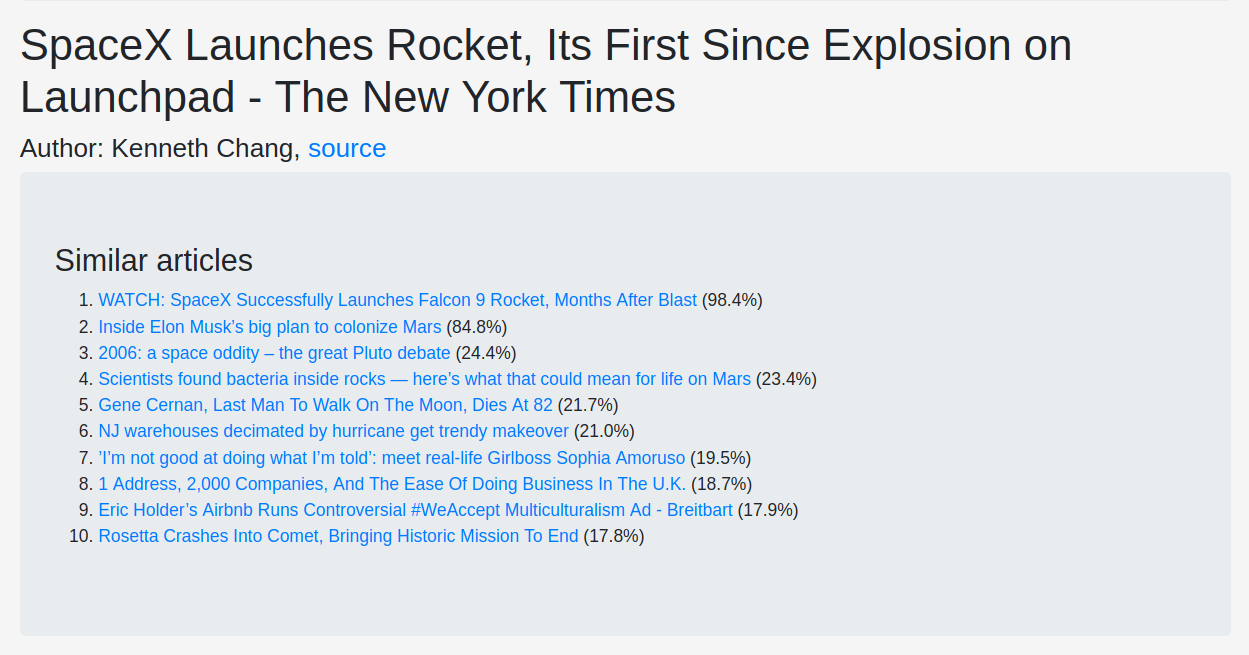
\includegraphics[width=0.9\columnwidth]{images/output.png}
	\caption{Příklad výstupu aplikace}
	\label{output}
\end{figure}

Na obrázku \ref{output} je vidět konkrétní vstup a výstup naší aplikace. Zobrazí se název článku dotazu, jméno jeho autora a také samotný text článku. Naše aplikace dále uživateli nabídne seznam 10 nejpodobnějších článků i s určenou kosinovou podobností v procentech. Je vidět, že aplikace vrací víceméně přesně to, co bychom čekali. K článku o tom, že firma SpaceX vypustila do vesmíru raketu, vrátí články týkající se firmy SpaceX či raket.

\section{Experimentální sekce}

\subsection{Určení optimálního počtu konceptů}

\begin{figure}[h] % [h] forces the figure to be output where it is defined in the code (it suppresses floating)
	\centering
	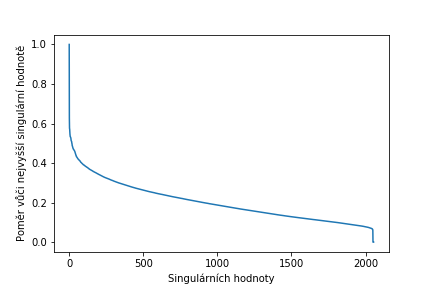
\includegraphics[width=0.7\columnwidth]{images/singular_values.png}
	\caption{Důležitost konceptů}
	\label{concepts}
\end{figure}

Vezmeme si singulární hodnoty, které nám vrátil singulární rozklad v rovnici \ref{eq:svd}. Vizualizujeme-li si v grafu \ref{concepts}, jak klesá poměr nejvyšší singulární hodnoty vůči zbylým singulárním hodnotám, vidíme z toho také, jak klesá důležitost konceptů v datasetu. Počet konceptů $k$ v naší aplikaci tedy podle tohoto grafu určíme jako 400.

\subsection{Porovnání vlivu LSI na kvalitu výsledků vyhledávání s ohledem na výskyt synonym a homonym}

Pro zjištění kvality výsledků vyhledávání s ohledem na výskyt synonym a homonym jsme do datasetu přidali 4 články.

\subsubsection{Synonyma}

Jak si náš model poradí se synonymy jsme testovali na článcích \emph{"Silicon Valley’s favorite magician reimagines his act in the age of Zoom"} a \emph{"Leading NYC Illusionist Launches Virtual Magic Shows"}. Testovali jsme tedy anglická synonyma \emph{illusionist} a \emph{magician}.

\begin{figure}[h] % [h] forces the figure to be output where it is defined in the code (it suppresses floating)
	\centering
	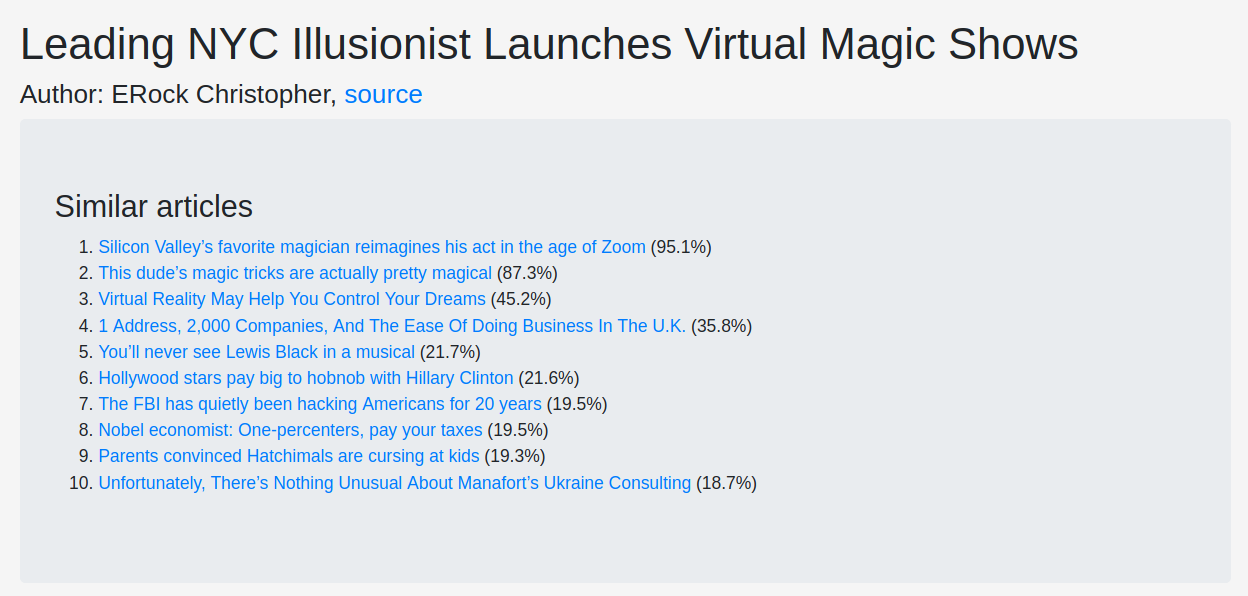
\includegraphics[width=0.8\columnwidth]{images/synonyms_0.png}
	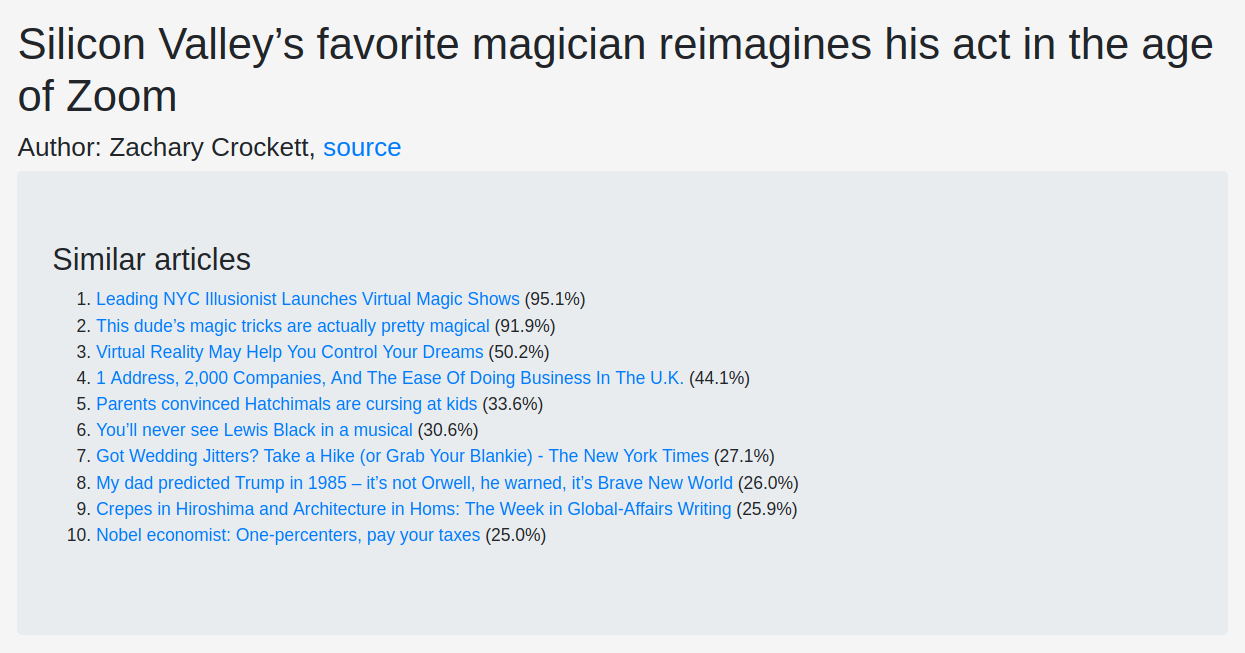
\includegraphics[width=0.8\columnwidth]{images/synonyms_1.png}
	\caption{Synonyma}
	\label{synonyms}
\end{figure}

\bigskip

Na obrázku \ref{synonyms} je vidět, že náš model synonyma v článcích identifikoval správně. V prvním článku se sice ani jednou přímo nevyskytuje slovo \emph{magician} a v druhém ani jednou slovo \emph{illusionist}, ale v obou se vyskytují slova se slovním záladem \emph{magic} nebo například slova \emph{show} a \emph{audience} a model tak články správně identifikoval jako podobné.

\subsubsection{Homonyma}

K testování jak si náš článek poradí s homonymy jsme použili články \emph{"Little Richard, rock 'n' roll pioneer, has died at 87"} a \emph{"Scientists found bacteria inside rocks — here’s what that could mean for life on Mars"}, které oba obsahují slovo \emph{rock} ovšem jednou ve významu skály a jednou ve významu rockového muzikanta.

\begin{figure}[h] % [h] forces the figure to be output where it is defined in the code (it suppresses floating)
	\centering
	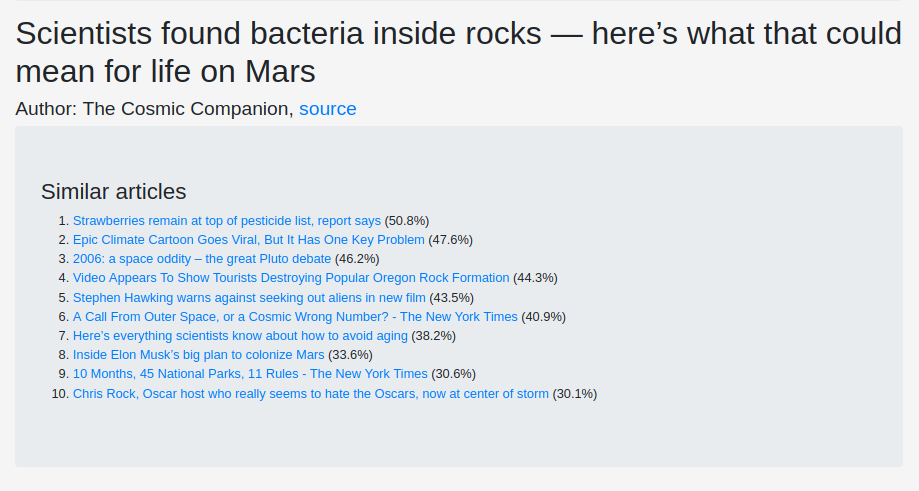
\includegraphics[width=0.8\columnwidth]{images/homonyms_0.png}
	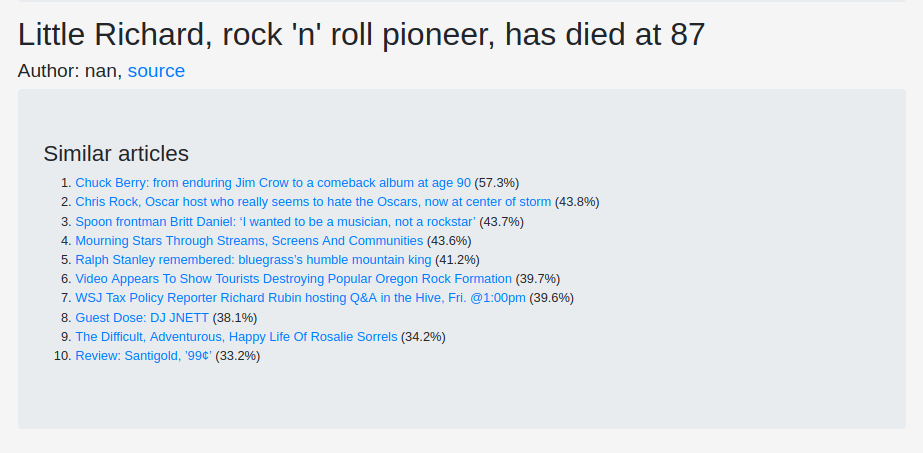
\includegraphics[width=0.8\columnwidth]{images/homonyms_1.png}
	\caption{Homonyma}
	\label{homonyms}
\end{figure}

\bigskip

Na obrázku \ref{homonyms} je vidět, že u prvního článku, týkajícího se vlivu objevu bakterie v podmořských skalách na možnost žvota na Marsu, si model poradil opravdu dobře a vrátil nám články týkající se vesmíru nebo přírody. Jediné co model spletlo je článek o Chrisi Rockovi, jehož příjmení, které se ve článku vyskytuje velmi často, jsme při předzpracování převedli na malá písmena do tvaru \emph{rock} a model tak neví, že se jedná o vlastní jméno. I přes tento problém jsme se v naší aplikaci rozhodli všechna slova převádět na malá písmena. Kdybychom se rozhodli převádět na malá písmena pouze slova na začátcích vět a ostatní vlastní jména nechávali s velkým písmenem na začátku, identifikoval by nám model například slovo \emph{school} a slovo \emph{School} v názvu nějaké školy jako 2 rozdílná slova. Je tedy na zvážení autorů aplikace, jak k problému přistoupí.

\bigskip

U druhého článku týkajícího se smrti rockového hudebníka nám jako první vrátil velmi relevantní článek o jiném stárnoucím hudebníkovi. Jako druhý článek nám model opět vrátil článek o Chrisi Rockovi, jež je teď pro model velmi relevantní, jelikož je to článek o celebritě a obsahuje spoustu výskytů slova \emph{rock}. Třetí, čtvrtý a pátý článek jsou opět relevantní články o hudebnícíh, ale jako šestý článek už model vrátí článek o skále namísto o hudebnících. Je tedy vidět, že velmi relevantní články o hudebnících model identifikuje správně jako nejpodobnější, u méně relevatních článků týkajících se hudebníků, hudby nebo celebrit už má model problém identifikovat, jestli jsou relevantnější tyto články nebo články o skalách. Velmi záleží na tom, kolik podobných slov se ve článcích vyskytuje.

\subsection{Porovnání průchodu pomocí LSI vektorového modelu se sekvenčním průchodem databáze s ohledem na čas vykonání dotazu}

Pro odsimulování sekvenčního průchodu databází nastavíme počet konceptů stejný jako počet dokumentů databáze. Toho docílíme tak, že v souboru \emph{server/lsa\_config.json} nastavíme parametr $k$ na 0.

\begin{figure}[h] % [h] forces the figure to be output where it is defined in the code (it suppresses floating)
	\centering
	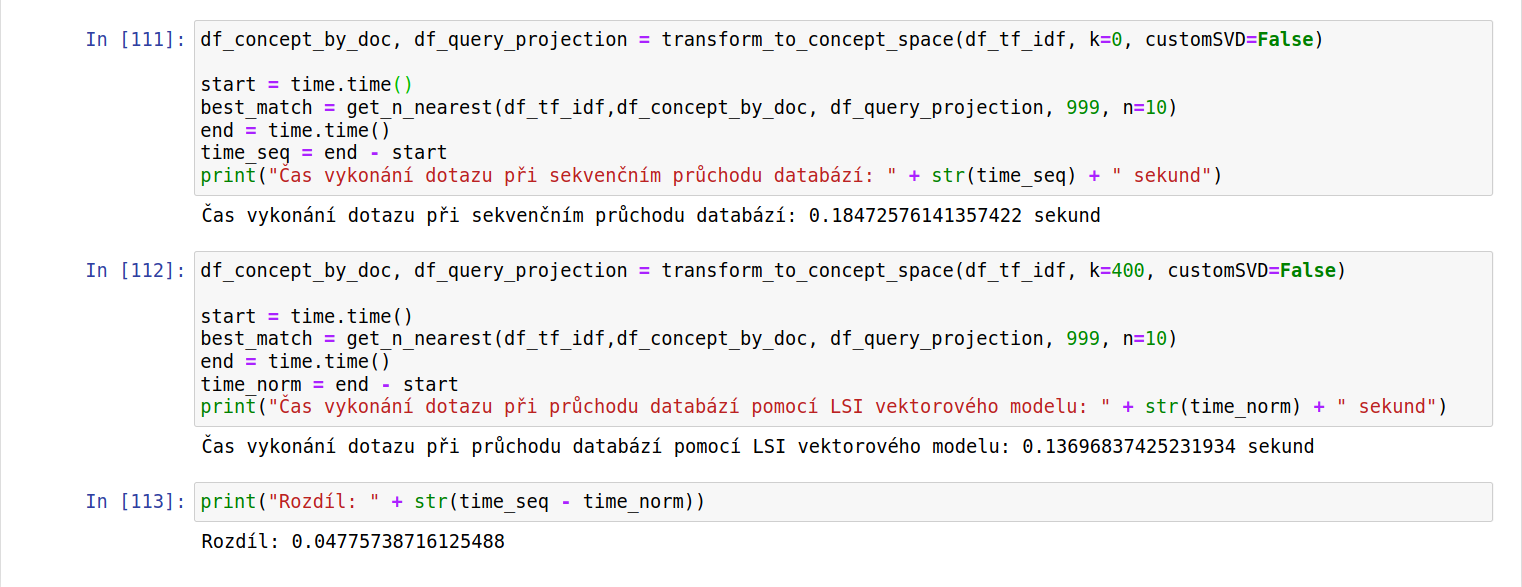
\includegraphics[width=1\columnwidth]{images/measure_time.png}
	\caption{Porovnání času vykonání dotazu při sekvenčním průchodu databáze}
	\label{measure_time}
\end{figure}

\bigskip

Na obrázku \ref{measure_time} je vidět, že při sekvenčním průchodu databází se čas vykonání dotazu zpomalí asi o
0.05 sekund. Při spuštění Flask serveru a testování v prohlížeči je však rozdíl v rychlosti načítání stránky zobrazující obsah článku a 10 jemu nejpodobnějších článku mnohem výraznější, kolem 3 sekund.

\subsection{Vliv různých vnitřních parametrů na výkon algoritmu (změna počtu konceptů, změna počtu extrahovaných termů, použití lemmatizace namísto stemmingu, odstranění číslovek při preprocesingu, použití jiného vzorce na výpočet vah termů...)}

\section{Diskuze}


\section{Závěr}

\end{document}
